\documentclass{beamer}
 
\usepackage[utf8]{inputenc}
\usepackage{etoolbox}
\usetheme{Copenhagen}
 
 
%Information to be included in the title page:

\logo{%
    \makebox[0.95\paperwidth]{%
        
\includegraphics[height=1.1cm,keepaspectratio]{pics/oeaw-logo.jpg}%
        \hfill%
        
\includegraphics[height=1.1cm,keepaspectratio]{pics/smi-logo.jpg}%
        \hspace*{3mm}
    }%
}

\title[Introduction to Machine learning] %optional
{Machine learning methods applied to the analysis of central exclusive production events in ALICE}
 
% \subtitle{A short story}
  
\author[Ratzenböck] % (optional, for multiple authors)
{Sebastian Ratzenböck\inst{1}}

\institute[SMI] % (optional)
{
\inst{1}%
Stefan Meyer Institut\\
Österreichische Akademie der Wissenschaften
}
  
\date[26.April 2018] % (optional)
{26. April 2018}
 
\begin{document}

%------------------------------------------------ 
\frame{\titlepage}

%------------------------------------------------ 

\begin{frame}
    \frametitle{Outline}
    \tableofcontents
\end{frame}

%------------------------------------------------ 
\section{ML: an overview} %

\begin{frame}
    \frametitle{ML: an overview}
    In general ML represents a contrast to a \emph{rule based systems}
    \begin{block}{Rule-based system}
        System that uses rules to make deductions or choices
        \begin{itemize}
            \item<1-> Domain-specific expert system
            \item<2-> Knowledge base: facts \& rules (if $\to$ then statement)
            \item<3-> Rules manually specified (by expert) $\to$ expensive, incomplete
        \end{itemize}
    \end{block}
\end{frame}

%------------------------------------------------ 

% \begin{frame}
%     \frametitle{ML: an overview}
%     In general ML represents a contrast to a \emph{rule based systems}
%     \begin{block}{Machine learning}
%         \begin{itemize}
%             \item<1-> Alorithms that learn from \emph{data} \& make predictions on \emph{data}
%             \item<2-> Automatic methods (no human needed)
%             \item<3-> Human work required for defining problem \& assessing the data
%         \end{itemize}
%     \end{block}
% \end{frame}

%------------------------------------------------ 

\begin{frame}
    \frametitle{ML: an overview}
    \vspace*{-7mm}
    In general ML represents a contrast to a \emph{rule based systems}
    \begin{columns}[T] % align columns
        \begin{column}{.48\textwidth}
            % \color{red}\rule{\linewidth}{4pt}
            \begin{block}{Machine learning}
                \begin{itemize}
                    \item<1-> Alorithms that learn from \emph{data} \& make predictions on \emph{data}
                    \item<2-> Automatic methods (no human needed)
                    \item<3-> Human work required for defining problem \& assessing the data
                \end{itemize}
            \end{block}
        \end{column}%
        \hfill%
        \begin{column}{.48\textwidth}
            % \color{blue}\rule{\linewidth}{4pt}
            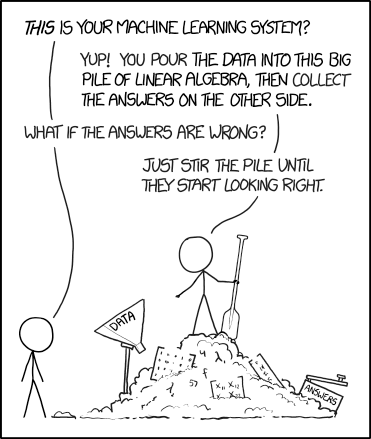
\includegraphics[height=5cm,keepaspectratio]{pics/machine_learning.png}%
            
        \end{column}%
    \end{columns}
\end{frame}

%------------------------------------------------ 

\begin{frame}
    \frametitle{Types of ML}
    \begin{columns}[T] % align columns
        \begin{column}{.35\textwidth}
            % \color{red}\rule{\linewidth}{4pt}
            \begin{itemize}
                \item Supervised 
                \begin{itemize}
                    \item Classification
                    \item Regression
                \end{itemize}
                \item Unsupervised
            \end{itemize}
        \end{column}%
        \hfill%
        \begin{column}{.7\textwidth}
            % \color{blue}\rule{\linewidth}{4pt}
            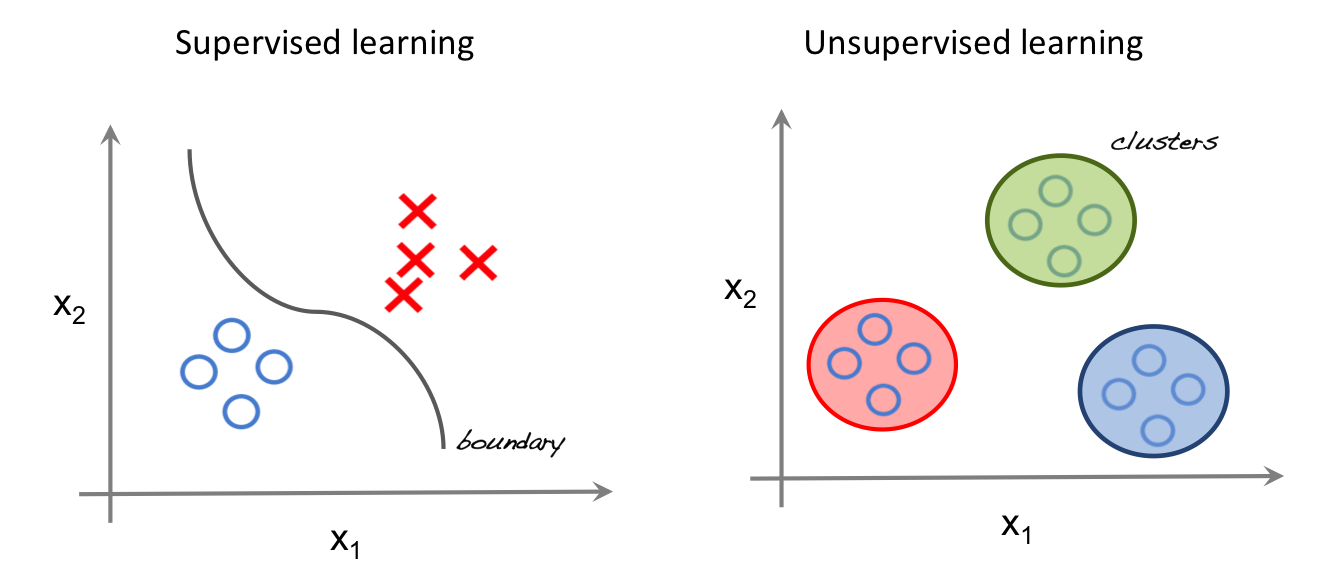
\includegraphics[height=3cm,keepaspectratio]{pics/supervised_vs_unsupervised.png}%
            
        \end{column}%
    \end{columns}
\end{frame}

%------------------------------------------------ 

\section{Recap: rectangular cuts} %
\begin{frame}
    \frametitle{Rectangular cuts}
\end{frame}

%------------------------------------------------ 


 
\end{document}



